\documentclass{article}
\usepackage{amsmath}
\usepackage{amssymb}
\usepackage{float}
\usepackage{graphicx}
\begin{document}
	\section[General]{General Form}
	A resistor-capacitor (RC) series circuit with a resistance of $R$ ohms, a 
	capacitance of $C$ farads, 
	and a power supply with a constant voltage of $V$ volts is of the general 
	form:
	\begin{equation}\label{eq:integro-diff-eq}
		Ri + \frac{1}{C}q = V
	\end{equation}
	Here, $i(t):=i$, denotes the amplitude of the current running through the 
	circuit measured in amps, while $q(t):=q$ denotes the charge in the 
	capacitor measured in Coloumbs.  The aforementioned charge is equal to the 
	primitive integral of $i(t)$.
	\begin{equation}\label{eq:charge}
		q = \int i \cdot dt
	\end{equation}
	Differentiating throughout equation (\ref{eq:integro-diff-eq}) with respect 
	to time gives the differential equation:
	\begin{equation}\label{eq:diff-eq}
		Ri' + \frac{1}{C}i = 0
	\end{equation}
	Multiplying throughout by $C$ gives:
	\begin{equation}\tag{\ref{eq:diff-eq}}
		CRi' + i = 0
	\end{equation}
	The most general solution for $i(t)$ is of the form:
	\begin{equation}\label{eq:current}
		i = Ae^{mt}
	\end{equation}
	where $A \in \mathbb{R}$ is an arbitrary constant to be solved for using 
	some initial value or boundary problem (IVP or IBP) involving the charge, 
	and $m$ is the root of the auxiliary equation (AE):
	\begin{equation}\label{eq:aux-eq}
		CRm + 1 = 0
	\end{equation}
	Via the above equation,
	\begin{equation}\tag{\ref{eq:aux-eq}}
		m = -\frac{1}{CR}
	\end{equation}
	And now, to solve for $A$, we will use the IVP,
	\begin{equation}\label{eq:ivp}
		q(0) = q_0
	\end{equation}
	First, we need to find an equation with the charge in terms of the 
	arbitrary constant that we are solving for.  Via equations 
	(\ref{eq:charge}) and (\ref{eq:current}),
	\begin{equation}\tag{\ref{eq:charge}}
		q = \frac{A}{m}e^{mt} + K	
	\end{equation}
	where $K \in \mathbb{R}$ is another arbitrary constant. \\ \\
	Via equations (\ref{eq:charge}) and (\ref{eq:ivp}),
	\begin{equation}\tag{\ref{eq:ivp}}
		\frac{A}{m} + K = q_0
	\end{equation}
	To solve for both arbitrary constants, we need two unique equations that 
	share at least one of the constants;  Additionally, at least 
	on of the equations must contain both of the aforementioned constants.  
	Thankfully, we are in luck! \\ \\
	Via equations (\ref{eq:integro-diff-eq}), (\ref{eq:current}), 
	(\ref{eq:charge}), and substitution,
	\begin{equation}\tag{\ref{eq:integro-diff-eq}}
		Ri(0) + \frac{1}{C}q(0) = RA + \frac{1}{C}\left(\frac{A}{m} + K\right) 
		= V
	\end{equation}
	The above equation allows us to solve for $K$ in terms of $A$.
	$$ \frac{A}{m} + K = C(V - RA)$$
	\begin{equation}\label{eq:K}
		K = C(V-RA) - \frac{A}{m}
	\end{equation}
	Via the above, equation (\ref{eq:ivp}), and substitution,
	$$ q_0 = C(V-RA)$$
	$$ V_C(0) = V-RA$$
	$$ RA = V-V_C(0)$$
	\begin{equation}\label{eq:A}
		A = R^{-1}(V - V_C(0))		
	\end{equation}
	\subsection{Examples}
	Herein are some examples.
	\begin{figure}[H]\label{fig:circuit}
		\caption{RC-Circuit with two resistors and a capacitor.}
		\centering
		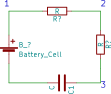
\includegraphics[width=0.75\linewidth,height=0.4\linewidth]{g1982}
	\end{figure}
	\subsection{Initial Charge}
	Via equations (\ref{eq:current}), (\ref{eq:A}), and substitution, it is 
	possible to find the initial charge, $q(0):=q_0$, assuming that the initial 
	current, $i(0):=i_0$, is known.
	$$ i(0) = A = R^{-1}(V-V_C(0))$$
	$$ Ri_0 = V- V_C(0)$$
	$$ V_C(0) = V - V_R(0)$$
\end{document}
